\chapter{On the production of entangled beams from a metastable Helium BEC}
\label{Peaks}
\graphicspath{{Figures/Peaks/}{Figures/Common/}}

The results presented in this chapter have been published in \citet{Dall:2009}. All of the theoretical work in this paper except as noted in this chapter was my own work.

\section{Introduction}
Sources of matter waves gained a dramatic improvement with the achievement of Bose-Einstein condensation (BEC) in dilute gases and the development of the atom laser \citep{Anderson:1995vn,Mewes:1997}. Like optical lasers before them, atom lasers can produce Heisenberg-limited beam profiles \citep{Busch:2002zr,Riou:2006uq} and promise high spectral density through their dramatically lower linewidth \citep{Wiseman:1997ba}. Another exciting possibility resulting from having such a coherent source of atoms is the generation of nonclassical matter waves through entangled beams. Such entangled beams are useful for tests of quantum mechanics and are required to perform Heisenberg-limited interferometry \citep{Dowling:1998,Reid:1988}. In this chapter, we show that the asymmetric scattering lengths between internal states of metastable helium (He*) cause well-defined peaks in the output of an atom laser. These peaks are due to a phase-matched four-wave mixing (FWM) process and are experimentally demonstrated.

A nonlinear process is required to produce entanglement, and one of the advantages of atomic systems over optical systems is that there are strong inherent nonlinearities due to atomic interactions, although these interactions can also lead to complications. These nonlinearities allow certain analogues of nonlinear optical experiments such as four-wave mixing (FWM) and Kerr squeezing to be performed directly in the atomic sample \citep{WallsMilburn}. All of these produce entanglement in optical systems. Four-wave mixing in a trapped BEC has been demonstrated experimentally in configurations where three distinct momentum states generated a fourth \citep{Deng:1999qy} and where two momentum states generated a pair of correlated atomic beams \citep{Vogels:2002}. These experiments demonstrated that the output phase was coherent, but the correlation properties were not measured. More recently the pair correlations in a spontaneous scattering of two colliding condensates were measured using the single-atom detectors available for He* atoms \citep{Perrin:2007}.

Using these existing sources of entangled pairs of atoms for interferometric experiments will be complicated by the high densities of the sources, where the nonlinearities that generated the correlations ultimately degrade the long-term coherence of the sample. While recent experiments have increased the coherence of atom interferometers by several orders of magnitude by reducing the nonlinearities with a Feschbach resonance \citep{Fattori:2008,Gustavsson:2008}, this precludes the production of entangled pairs. In our scheme the nonlinear interactions are used to drive FWM in the magnetically untrapped condensate, but the resulting untrapped beams that propagate in free space are dilute, potentially avoiding the decoherence problem. We show that pairs of beams can be produced simply by the process of radio-frequency (rf) outcoupling from a He* BEC, without the need for Feschbach resonances, optical traps, or scattering pulses. Unlike previous methods, which required pairs of atoms travelling at high kinetic energies as a source, this process involves scattering between atoms initially in the same zero-momentum state to create states with nonzero momentum. Semiclassical and field-theoretic simulations of the experiment show that the beams are generated by the same FWM process that generated entangled atom pairs in the earlier experiments.

\section{The metastable Helium `Peaks' experiment}
\label{Peaks:ExperimentalSetup}

The experimental setup for creating He* BEC has been reported elsewhere \citep{Dall:2007a}, and discussed earlier in this thesis (see \sectionref{He*Experiment}\footnote{FIXME: Correct this reference when this section is written}).

Starting from an almost pure BEC containing up to $5\times 10^6$ atoms an atom laser beam was created by using rf photons to spin flip the BEC atoms from the $m=1$ magnetically trapped state to the $m=0$ untrapped state.

After outcoupling, atoms in the atom laser beam fell under gravity for a distance of $\unit[4]{cm}$ until they hit a double stacked multichannel plate (MCP). The phosphor screen was imaged with a charge-coupled-device (CCD) camera with a resolution of approximately $\unit[150]{\micro m}$ at the MCP. To remove any nonuniformities caused by spatial variations in the gain of the MCP, all images were divided by a flat-field image produced by dropping atoms from a MOT onto the detector. Since the MOT temperature is of order $\sim\unit[1]{mK}$, the spatial profile of the MOT uniformly illuminates the MCP. Although $m=-1$ atoms are produced by the outcoupling, especially for high rf powers, they are in general accelerated away from the detector by the magnetic trap field. Those that are accelerated towards the detector do not show up in the images since they arrive much earlier than the CCD trigger time.

\figureref{Peaks:ExperimentalResults} shows the dramatic change in the atom laser spatial profile when the condensate undergoes the resonant FWM process. In the case of low outcoupling Rabi frequencies (upper row), the FWM process does not occur and we see the usual double-peaked He*-atom laser profile \citep{Dall:2007} (see also \sectionref{TransverseProfile:Helium}\footnote{FIXME: Correct this reference when this section is written}). When the Rabi frequencies are high enough to initiate the FWM process (lower row), the atoms in the atom laser beam are scattered to form a halo around the main atom laser beam. Due to conservation of energy, the outer diameter of this halo corresponds to a maximum kinetic energy given by the chemical potential. As well as the ring structure, four peaks are observed on the outskirts of the profile.
% Each peak contains 11\%--14\% of the total outcoupled atoms, in agreement with the value of 11\% obtained from the simulation results shown in the lower row of \figureref{Peaks:ExperimentalResults}.

These peaks arise from two momentum-correlated cones of particles scattering out of the condensate and falling to the detector, as shown in \figureref{Peaks:Schematic}. The cones themselves are generated by a dynamical instability that populates momentum modes lying along the weak trapping axis, which expand to rings due to the mean-field repulsion in the tight trapping direction as they leave the BEC. Atoms in these cones then fall under gravity onto the detector, where the time-integrated flux is converted to a spatial density distribution, and each momentum ring appears as a double peak. The background halo is produced during the initial switch-on of the atom laser during which the peaks produced by the FWM process sweep in position from the main atom laser profile towards their final position in \figureref{Peaks:ExperimentalResults}.

\begin{figure}[htbp]
    \centering
        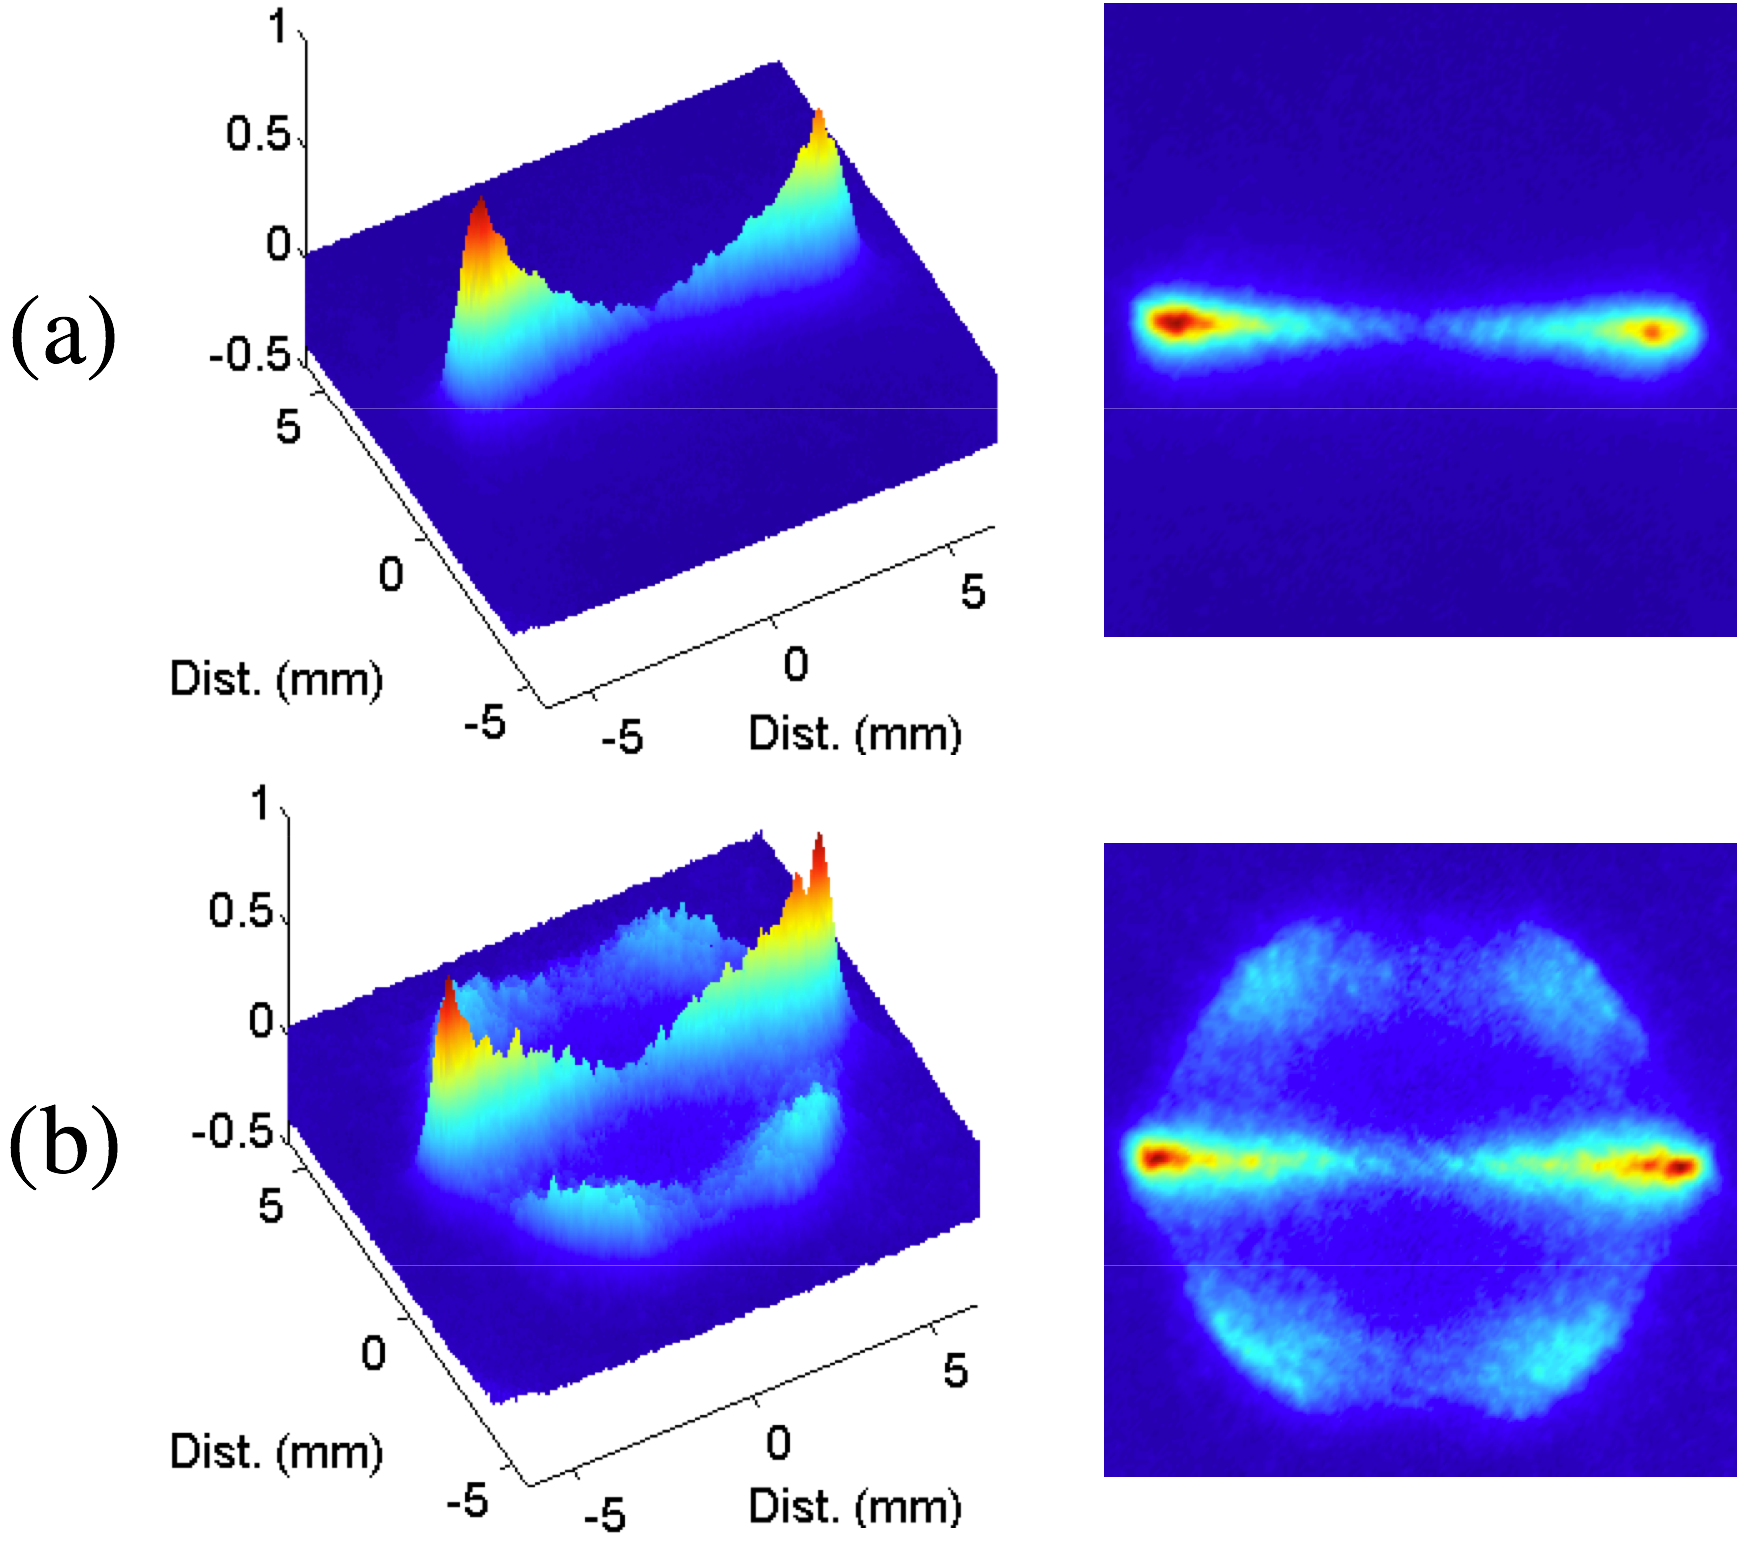
\includegraphics[height=3in]{ExperimentalResults}
    \caption{Experimental results. The difference between (a) and (b) is that the outcoupling Rabi frequency has been increased by an order of magnitude in (b).}
    \label{Peaks:ExperimentalResults}
\end{figure}

\begin{figure}[htbp]
    \centering
        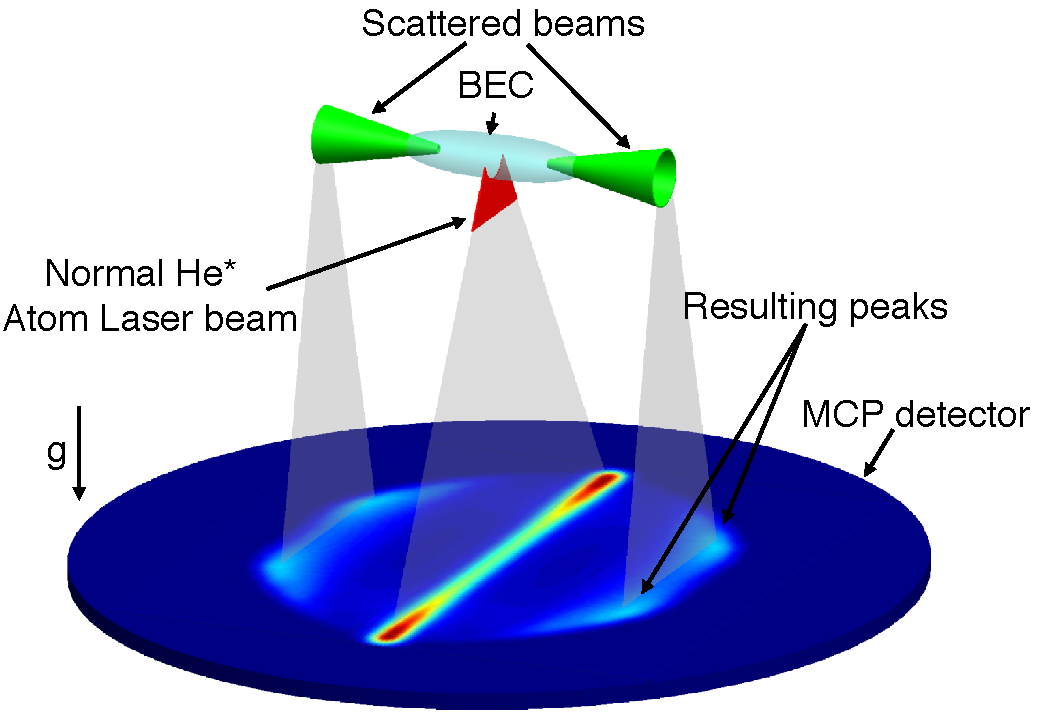
\includegraphics[height=3in]{Schematic}
    \caption{Schematic of the experimental setup}
    \label{Peaks:Schematic}
\end{figure}


\begin{table}
    \centering
    \begin{tabular}{cc}
    \toprule
    Parameter & Value\\
    \midrule
    Condensate number & $N = 2\times 10^6$\\
    Radial trapping frequency & $\omega_\rho = 2 \pi \times \unit[1020]{Hz}$\\
    Axial trapping frequency & $\omega_z = 2\pi \times \unit[55]{Hz}$\\
    Outcoupling Rabi frequency & $\Omega = 2\pi \times \unit[3]{kHz}$\\
    \bottomrule
    \end{tabular}
    \caption{Experimental parameters for the metastable Helium BEC under consideration.}
    \label{Peaks:ExperimentalParameters}
\end{table}

\clearpage
\section{Condensate excitations in the perturbative regime}
\label{Peaks:PerturbativeApproach}
%While the argument in the previous section gives a qualitative explanation for the four-wave mixing process observed in He*, it is not entirely satisfying. In this section an approximate analytic expression for the excited modes of the He* system will be obtained and investigated using Bogoliubov stuff.

The observed features in the atom laser profile presented in the previous section are caused by a dynamical instability in the condensate that causes the formation of momentum excitations in a narrow range of momenta along the weak trapping axis. During outcoupling these excitations are accelerated along the tight trapping directions forming the momentum cones pictured in \figureref{Peaks:Schematic}. The detection process vertically integrates this momentum profile leading to the observed peaks in \figureref{Peaks:ExperimentalResults}.
% The background halo between these peaks and the usual atom laser profile is the result of (at higher detunings resonant momentum will vary across surfaces, during this initial switch-on phase, a range of momenta are excited)\footnote{FIXME: Complete and correct this sentence.}.

The dynamical instability is due to the significantly different scattering lengths between the Zeeman levels of He*. In a later section a full multimode quantum-field calculation will be discussed and its results presented, but it is enlightening to first consider a simplified model in which the energy spectrum (and stability) of small excitations to the condensate can be obtained.

The simplified model to be considered is that of a homogenous spinor condensate consisting of two levels with Rabi oscillations coupling the two levels. The approximation that the condensate is homogenous (known as the local density approximation \cite{Stamper-Kurn:1999,Zambelli:2000}) is justified if the excitations under considerations have wavelengths much smaller than the Thomas-Fermi radius in that dimension. The local density approximation will hold for this system along the axial direction as the axial momentum of the features observed in \figureref{Peaks:ExperimentalResults} corresponds to an excitation wavelength of $\sim \unit[5]{\micro m}$, significantly smaller than the Thomas-Fermi radius in the axial direction of $z_\text{TF} = \unit[175]{\micro m}$. 

The second approximation made in this model is to neglect the antitrapped state $m_F=-1$. Any density in this state leaves the condensate very rapidly due to the combined effects of both the mean-field repulsion and the magnetic field gradient. A classical particle in the centre of the condensate under the influence of the same effective potential experienced by the $m_F=-1$ atoms would reach a momentum equal to the momentum width of the condensate (and hence no longer be able to couple to the stationary atoms in the middle of the condensate) in $\sim\unit[80]{\micro s}$, significantly shorter than the inverse Rabi frequency of $\sim \unit[300]{\micro s}$.

With these approximations made, the Hamiltonian for this system is
\begin{align}
    \label{Peaks:InitialHamiltonian}
    \begin{split}
    \hat{H} &= \sum_i \int d\bm{x}\, \hat{\Psi}_i^\dagger \left(\frac{-\hbar^2 \nabla^2}{2 M} - \mu\right)\hat{\Psi}_i^{} + \frac{1}{2} \sum_{i j} U_{i j}\int d\bm{x}\, \hat{\Psi}_i^\dagger \hat{\Psi}_j^\dagger \hat{\Psi}_j^{} \hat{\Psi}_i^{}\\
            &\phantom{=} + \hbar \Omega \int d\bm{x}\, \left(\hat{\Psi}_1^\dagger \hat{\Psi}_0^{} + \hat{\Psi}_0^\dagger \hat{\Psi}_1^{}\right),
    \end{split}
\end{align}
where $U_{ij} = 4\pi \hbar^2 a_{ij}/M$ is the nonlinear interaction strength, $a_{ij}$ is the s-wave scattering length between internal states $i$ and $j$, $\Omega$ is the Rabi frequency which is taken to be real, and $\mu$ is an energy offset which has been included to cancel the global phase rotation which would otherwise be present. The equations of motion corresponding to this Hamiltonian are
\begin{subequations}
    \label{Peaks:OperatorEquationsOfMotion}
    \begin{align}
    i \hbar \frac{\partial \hat{\Psi}_1}{\partial t}  &= -\frac{\hbar^2}{2M}\nabla^2 \hat{\Psi}_1  + U \left(\hat{\Psi}_1^\dagger \hat{\Psi}_1^{} + \hat{\Psi}_0^\dagger \hat{\Psi}_0^{}\right) \hat{\Psi}_1^{} + \hbar \Omega \hat{\Psi}_0^{} - \mu \hat{\Psi}_1^{},  \\
    i \hbar \frac{\partial \hat{\Psi}_0}{\partial t} &= -\frac{\hbar^2}{2M} \nabla^2 \hat{\Psi}_0 + U \left(\hat{\Psi}_1^\dagger \hat{\Psi}_1^{} + \kappa \hat{\Psi}_0^\dagger \hat{\Psi}_0^{} \right) \hat{\Psi}_0^{} + \hbar \Omega \hat{\Psi}_1^{} - \mu \hat{\Psi}_0^{},
    \end{align}
\end{subequations}
where $U=U_{11}=U_{10}$ and $\kappa = U_{00}/U_{11}$. For metastable Helium in the $F=1$ manifold, $\protect{\kappa \approx 0.74}$\footnote{FIXME: Cite something.}, while for Rubidium in the $F=1$ manifold, $\kappa \approx 1.01$ \cite{Ho:1998}\footnote{FIXME: A more recent reference might be useful.}. 

\subsection{The dynamical steady-state}
\label{Peaks:MeanFieldPeriodicity}

The excitation spectrum of a condensate can be obtained by approximating each field operator to be a c-number (the mean-field) plus a small fluctuation term, and then either diagonalising the Hamiltonian \cite{Bogoliubov:1947,FetterWalecka} or diagonalising the linearised equations of motion for the fluctuations themselves (see, for example \cite{Ho:1998}\footnote{FIXME: Probably need an earlier and/or better reference here.}). It is the latter approach that will be taken here, but with the difference that the mean-field about which the linearisation procedure will take place is itself time-dependent.

The mean-field state that we wish to consider is one that corresponds to the state of the BEC in the experiment. At $t=0$ all of the population in this state will be in the $m_F=1$ level, representing the original trapped BEC, while the $m_F=0$ atom laser level will be initially unpopulated. Rabi oscillations will transfer population between these two levels, and it will be shown that these oscillations are periodic.

The method for diagonalising the evolution equations of the linearised fluctuations to obtain the excitation spectrum is the same method used to determine the stability of fixed points of systems of nonlinear ordinary differential equations. This method relies critically on the fact that it is a \emph{fixed} point about which the equations are linearised. Floquet's Theorem \citep{Nayfeh:1995} allows the stability of \emph{periodic} solutions to be considered, and it is this theorem that will be used to determine the stability of the mean-field evolution. It will now be shown that this mean-field evolution is periodic.

Within the local density approximation we can assume that the mean-field remains homogeneous; only the excitations will have spatial dependence. The equations of motion for the mean-field then reduce to the following ordinary differential equations,
\begin{subequations}
    \label{Peaks:MeanFieldEquationsOfMotion}
    \begin{align}
    i \hbar \frac{d \Psi_1}{dt} &= U\left(\abs{\Psi_1}^2 + \abs{\Psi_0}^2\right)\Psi_1 + \hbar \Omega \Psi_0 - \mu \Psi_1,\\
    i \hbar \frac{d \Psi_0}{dt} &= U\left(\abs{\Psi_1}^2 + \kappa \abs{\Psi_0}^2\right)\Psi_0 + \hbar \Omega \Psi_1 - \mu \Psi_0.
    \end{align}
\end{subequations}

Although solving \eqref{Peaks:MeanFieldEquationsOfMotion} for $\kappa \neq 1$ is intractable analytically, it can at least be shown that the solutions are periodic. This can be shown by recognising these equations as modified optical Bloch equations containing a nonlinear term but with no damping. Defining $\Psi_i = c_i\sqrt{n}$ where $n = \abs{\Psi_1}^2 + \abs{\Psi_0}^2$ is the total density, the equations of motion for the density matrix terms $\rho_{10} = c_{1}^{}c_{0}^*$ and $w = \rho_{11}-\rho_{00} = \abs{c_1}^2 - \abs{c_0}^2$ are
\begin{subequations}
    \label{Peaks:OpticalBlochEquations}
    \begin{align}
        \frac{d\rho_{10}}{dt} &= -i\frac{g}{2} (1-w)\rho_{10} + i \Omega w,\\
        \frac{d w}{dt} &= -4 \Omega \Im\{\rho_{10}\},
    \end{align}
\end{subequations}
where $g = n U (1-\kappa)/\hbar$. As the evolution is purely Hamiltonian, these equations will conserve the energy of the state. Up to an arbitrary additive constant, the energy per particle is given by
\begin{align}
    E &= -\frac{1}{8}\hbar g(1 - w)^2 + 2 \hbar \Omega \Re\{\rho_{10}\}.
    \label{Peaks:OpticalBlochEnergy}
\end{align}
The solutions to \eqref{Peaks:OpticalBlochEquations} are visualised in \figureref{Peaks:BlochSphere}.

As the evolution is purely Hamiltonian, the state can be described by a point on the surface of the Bloch sphere (see \figureref{Peaks:BlochSphere}).  The state is however not completely free to move on this sphere as the Hamiltonian must be conserved by its motion. This further restricts the system's motion to closed lines on the surface of the Bloch sphere, therefore requiring the system's motion to be periodic. Although this demonstrates that all physical expectation values are periodic, for the wavefunctions themselves to be periodic, the global phase rotation must be cancelled. This can be achieved by appropriate choice of the energy offset $\mu$. It is the periodicity of the wavefunctions $\Psi_i$ that will enable the stability of the condensate to excitations to be determined.

\begin{figure}
    \centering
    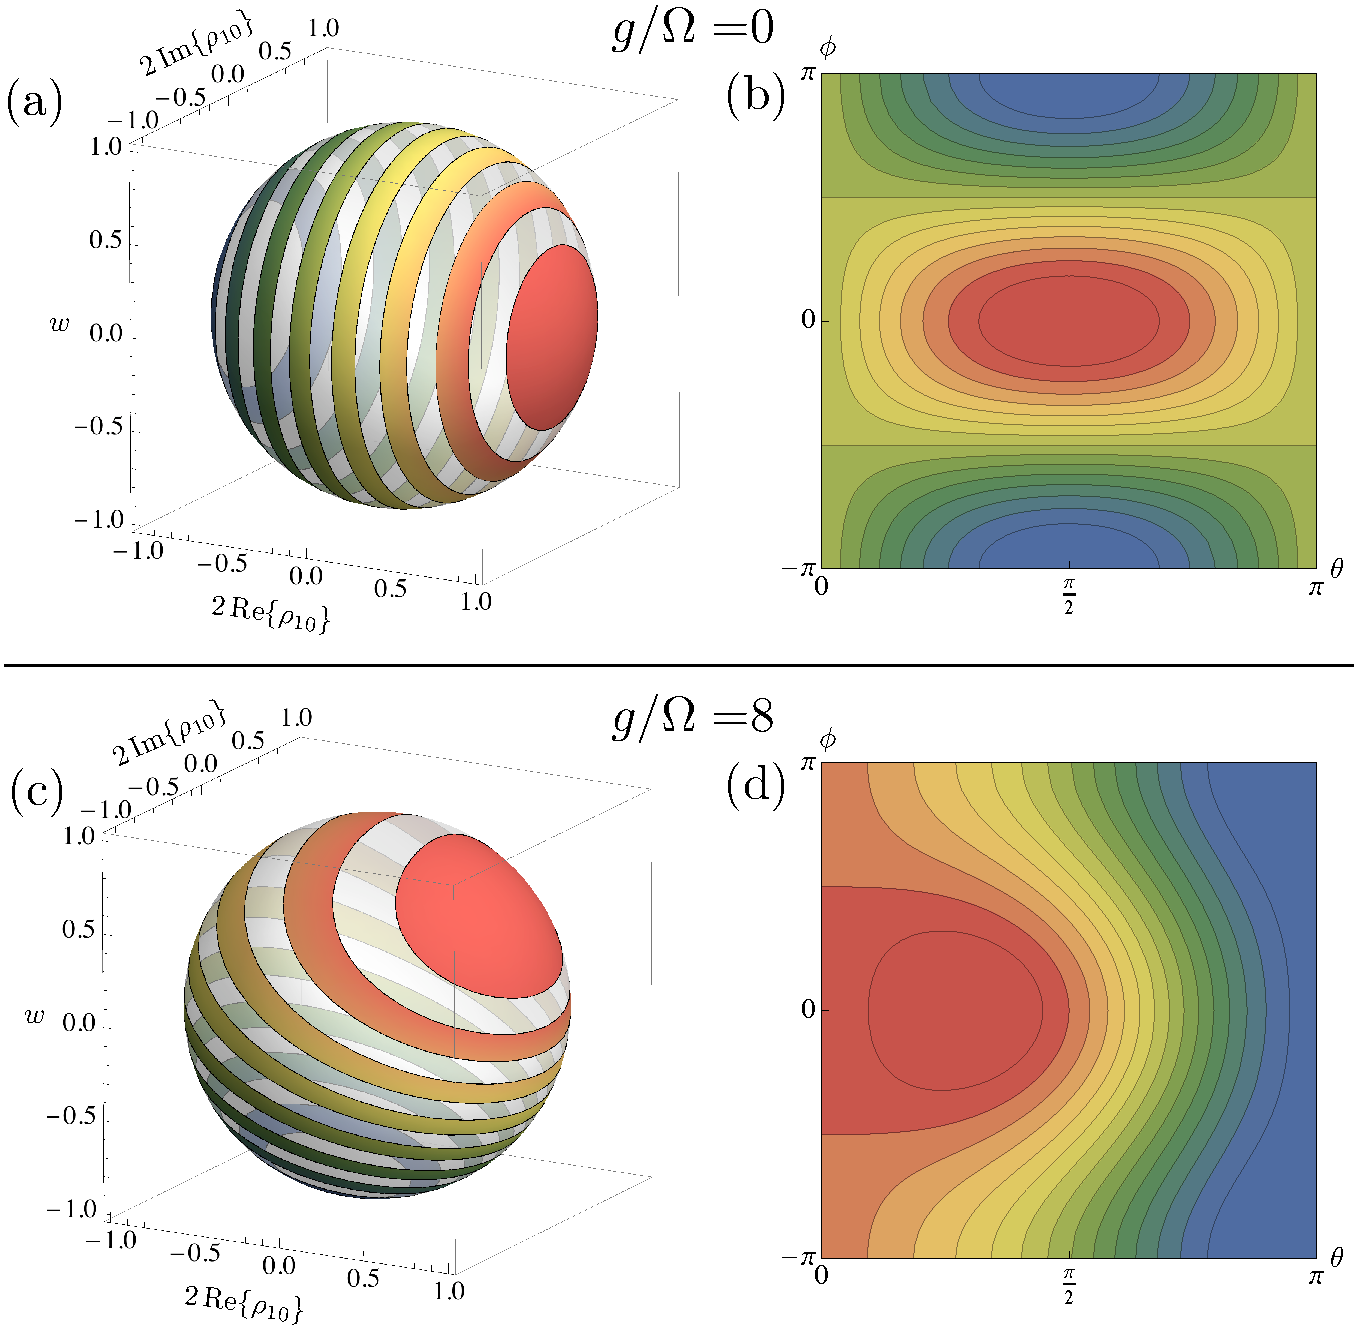
\includegraphics[width=14cm]{BlochSpheres}
    \caption{Bloch sphere representation of the evolution described by \eqref{Peaks:OpticalBlochEquations}. The upper figures (a) and (b) represent the case of the usual optical Bloch equations with no damping ($g/\Omega=0$), the lower figures (c) and (d) illustrate the effect of the nonlinear term on the evolution with $g/\Omega = 8$. The left figures (a) and (c) illustrate the Bloch sphere coloured according to the energy $E$ [see \eqref{Peaks:OpticalBlochEnergy}]. The system is constrained to move on lines of constant colour. Bands have been removed from these spheres for illustration purposes only. The right figures (b) and (d) are contour plots of the energy $E$ over the surface of the Bloch sphere.
     \label{Peaks:BlochSphere}}
\end{figure}

\subsection{Excitation dynamics}

The evolution of small perturbations about the mean-field dynamics of a condensate define both the excitation spectrum of the condensate and its stability to perturbations. 
%These perturbations not only arise from experimental uncertainties, but are an  inescapable consequence of quantum mechanics due to the fluctuations of the vacuum itself.
To determine the evolution of these excitations the mean-field dynamics must be separated from that of the excitations. To this aim we define the deviation operators $\delta\hat{\Psi}_i = \hat{\Psi}_i - \mean{\hat{\Psi}_i}$ and treat $\delta\hat{\Psi}_i$ as a small quantity. In this case the $\mean{\hat{\Psi}_i}=\Psi_i$ are themselves time dependent, obeying the equations for the mean-field, \eqref{Peaks:MeanFieldEquationsOfMotion}.

The equations of motion for the deviation operators are obtained by replacing the field operators $\hat{\Psi}_i$ in the operator evolution equations \eqref{Peaks:OperatorEquationsOfMotion} with $\Psi_i + \delta \hat{\Psi}_i$ and keeping only terms up to first order in the deviation operators. Applying this procedure gives
\begin{subequations}
    \label{Peaks:DeviationOperatorsEvolutionXSpace}
    \begin{align}
        \begin{split}
            i \hbar \frac{\partial \delta \hat{\Psi}_1}{\partial t} =& U\left[ \left(2\abs{\Psi_1}^2+\abs{\Psi_0}^2 \right)\delta \hat{\Psi}_1 + \Psi_1^2\delta\hat{\Psi}_1^\dagger + \Psi_1\Psi_0\delta\hat{\Psi}_0^\dagger + \Psi_0^*\Psi_1\delta\hat{\Psi}_0\right]\\
                    & - \frac{\hbar^2}{2M}\nabla^2 \delta \hat{\Psi}_1 +\hbar \Omega\delta\hat{\Psi}_0- \mu \delta \hat{\Psi}_1,
        \end{split}\\
        \begin{split}
        i \hbar \frac{\partial \delta \hat{\Psi}_0}{\partial t} =& U\left[\left(2\kappa \abs{\Psi_0}^2 +\abs{\Psi_1}^2\right)\delta\hat{\Psi}_0 + \kappa \Psi_0^2 \delta\hat{\Psi}_0^\dagger + \Psi_1\Psi_0\delta\hat{\Psi}_1^\dagger + \Psi_1^*\Psi_0\delta\hat{\Psi}_1\right]\\
                    & -\frac{\hbar^2}{2M}\nabla^2 \delta \hat{\Psi}_0 +\hbar \Omega\delta\hat{\Psi}_1 - \mu \delta\hat{\Psi}_0.
        \end{split}
    \end{align}
\end{subequations}

Having assumed the condensate to be homogenous, the system is translation-invariant and the evolution equations will take their simplest form in a Fourier basis. Performing the Fourier transform of \eqref{Peaks:DeviationOperatorsEvolutionXSpace} yields
\begin{subequations}
    \label{Peaks:DeviationOperatorsEvolutionKSpace}
    \begin{align}
        \begin{split}
            i \hbar \frac{\partial \delta \hat{\Psi}_1(\bm{k})}{\partial t} =& U\left[ \left(2\abs{\Psi_1}^2+\abs{\Psi_0}^2 \right)\delta \hat{\Psi}_1(\bm{k}) + \Psi_1^2\delta\hat{\Psi}_1^\dagger(-\bm{k}) + \Psi_1\Psi_0\delta\hat{\Psi}_0^\dagger(-\bm{k}) + \Psi_0^*\Psi_1\delta\hat{\Psi}_0(\bm{k})\right]\\
                    & +\frac{\hbar^2 \bm{k}^2}{2M} \delta \hat{\Psi}_1(\bm{k}) +\hbar \Omega\delta\hat{\Psi}_0(\bm{k})- \mu \delta \hat{\Psi}_1(\bm{k}),
        \end{split}\\
        \begin{split}
        i \hbar \frac{\partial \delta \hat{\Psi}_0(\bm{k})}{\partial t} =& U\left[\left(2\kappa \abs{\Psi_0}^2 +\abs{\Psi_1}^2\right)\delta\hat{\Psi}_0(\bm{k}) + \kappa \Psi_0^2 \delta\hat{\Psi}_0^\dagger(-\bm{k}) + \Psi_1\Psi_0\delta\hat{\Psi}_1^\dagger(-\bm{k}) + \Psi_1^*\Psi_0\delta\hat{\Psi}_1(\bm{k})\right]\\
                    & +\frac{\hbar^2 \bm{k}^2}{2M} \delta \hat{\Psi}_0(\bm{k}) +\hbar \Omega\delta\hat{\Psi}_1(\bm{k}) - \mu \delta\hat{\Psi}_0(\bm{k}).
        \end{split}
    \end{align}
\end{subequations}

In this form, it is clear that the Fourier modes are almost completely decoupled from each other. Each deviation operator $\delta\hat{\Psi}_i(\bm{k})$ is only coupled to $\left\{\delta\hat{\Psi}_j(\bm{k}),\, \delta\hat{\Psi}_j^\dagger(-\bm{k})\right\}$, with each $\delta\hat{\Psi}_i^\dagger(-\bm{k})$ also only coupled to this same set. This can be exploited to write the equations \eqref{Peaks:DeviationOperatorsEvolutionKSpace} in matrix form as
\begin{align}
    \label{Peaks:DeviationOperatorsMatrixEvolution}
    i \hbar \frac{\partial \hat{\bm{\Upsilon}}(\bm{k})}{\partial t} &= \mathcal{H}(\bm{k}) \hat{\bm{\Upsilon}}(\bm{k}),
\end{align}
where
\begin{align}
    \hat{\bm{\Upsilon}}(\bm{k}) &= 
    \begin{pmatrix}
        \delta\hat{\Psi}_1(\bm{k}) &
        \delta\hat{\Psi}_1^\dagger(-\bm{k}) &
        \delta\hat{\Psi}_0(\bm{k}) &
        \delta\hat{\Psi}_0^\dagger(-\bm{k})
    \end{pmatrix}^\text{T},\\
    \mathcal{H}(\bm{k}) &= 
    \begin{pmatrix}
        \varepsilon(\bm{k}) + q_{1} - \mu & v_{11} & u_{01} + \hbar \Omega & v_{10}\\
        -v_{11}^* & -\varepsilon(\bm{k}) - q_1 + \mu & -v_{10}^* & -u_{10} - \hbar \Omega\\
        u_{10} + \hbar \Omega & v_{10} & \varepsilon(\bm{k}) + q_0 - \mu & \kappa v_{00}\\
        -v_{10}^* & -u_{01} - \hbar \Omega & -\kappa v_{00}^* & -\varepsilon(\bm{k}) - q_0 + \mu
    \end{pmatrix},\label{Peaks:HMatrix}
\end{align}
and $q_1 = U\left(2\abs{\Psi_1}^2+\abs{\Psi_0}^2\right)$, $q_0 = U\left(2\kappa \abs{\Psi_0}^2 + \abs{\Psi_1}^2\right)$, $u_{ij} = U\Psi_i^*\Psi_j$, $v_{ij} = U\Psi_i\Psi_j$, and $\displaystyle \protect{\varepsilon(\bm{k}) = \frac{\hbar^2 \bm{k}^2}{2M}}$.

If the coefficients of the matrix $\mathcal{H}(\bm{k})$ were not time-dependent, the excitation spectrum of the condensate could simply be obtained from the real parts of the eigenvalues of $\mathcal{H}(\bm{k})$. Non-zero imaginary components for these eigenvalues would indicate the corresponding mode to be unstable\footnote{FIXME: Do these statements need more detail? Including it would detract from overall flow though.}. Before continuing with the general case of $\kappa \neq 1$, in the next section the limit in which all scattering lengths are equal ($\kappa=1$) will be considered and some familiar results recovered.

\subsection{Excitation spectra in the $\kappa = 1$ limit}
\label{Peaks:Kappa1Limit}
In the limit that all the scattering lengths are the same ($\kappa = 1$), the nonlinear term in \eqref{Peaks:MeanFieldEquationsOfMotion} only contributes to a rotation of the global phase of the spinor condensate. In this case the dynamics can be solved analytically and familiar excitation spectra recovered.

The general solution to \eqref{Peaks:MeanFieldEquationsOfMotion} for $\kappa = 1$ is
\begin{subequations}
    \label{Peaks:Kappa1MeanFieldSolution}
    \begin{align}
        \Psi_1(t) &= \cos(\Omega t) \Phi_+ + \sin(\Omega t) \Phi_-, \\
        \Psi_0(t) &= -i\sin(\Omega t) \Phi_+ + i\cos(\Omega t) \Phi_-,
    \end{align}
\end{subequations}
for some complex constants $\Phi_\pm$, and where the chemical potential $\mu = n U$ has cancelled the global phase rotation. This solution can be viewed as a linear basis transformation from $\Psi_i$ to $\Phi_\pm$. Performing this change of basis for both the $\Psi_i$ and $\delta \hat{\Psi}_i$ yields a matrix of precisely the same form as in \eqref{Peaks:HMatrix} but in terms of $\Phi_\pm$ instead of the $\Psi_i$, and with $\Omega \rightarrow 0$. This new matrix $\mathcal{H}'(\bm{k})$ is now time-independent and can be diagonalised to give the eigenvalues
\begin{subequations}
    \label{Peaks:Kappa1Eigenvalues}
    \begin{align}
        \hbar \omega_\uparrow(\bm{k}) &= \sqrt{\varepsilon(\bm{k})\left(\varepsilon(\bm{k}) + 2 n U\right)},\\
        \hbar \omega_\downarrow(\bm{k}) &= \varepsilon(\bm{k}),
    \end{align}
\end{subequations}
where $\displaystyle\varepsilon(\bm{k}) = \frac{\hbar^2\bm{k}^2}{2M}$, $n= \abs{\Psi_1}^2 + \abs{\Psi_0}^2$ and the remaining two eigenvalues are the negatives of \eqref{Peaks:Kappa1Eigenvalues}. $\hbar \omega_\uparrow(\bm{k})$ is the usual Bogoliubov spectrum \citep{Bogoliubov:1947} corresponding to excitations in the total condensate density. The eigenvalue $\hbar \omega_\downarrow(\bm{k})$ is the free particle spectrum; this excitation only changes the relative densities of the two states without affecting the total density, hence not affecting the nonlinear term in the Hamiltonian \eqref{Peaks:InitialHamiltonian}.

The Hamiltonian for the condensate excitations that corresponds to the eigenvalues \eqref{Peaks:Kappa1Eigenvalues} is
\begin{align}
    \hat{H} &= \sum_{i=\uparrow,\downarrow}\int d\bm{k}\, \hbar \omega_i(\bm{k}) \hat{\Lambda}_i^\dagger(\bm{k}) \hat{\Lambda}_i(\bm{k}),
\end{align}
where the $\hat{\Lambda}_{\uparrow,\downarrow}(\bm{k})$ obey boson commutation relations and are the corresponding normalised eigenvectors to the eigenvalues in \eqref{Peaks:Kappa1Eigenvalues}. The normalised eigenvectors for the negatives of those eigenvalues are the $\hat{\Lambda}_{\uparrow, \downarrow}^\dagger(-\bm{k})$.

\subsection[Floquet's theorem]{Floquet's theorem \citep{Nayfeh:1995}}
\label{Peaks:FloquetsTheorem}

Having considered the limit of equal scattering lengths, it now remains to determine the energy spectrum and condensate stability in the general case of $\kappa \neq 1$. Analytic results cannot be obtained in this limit, but numeric results corresponding to the experimental situation in \sectionref{Peaks:ExperimentalSetup} can be obtained.

In the general case, the excitation spectrum cannot be obtained from the eigenvalues of the matrix $\mathcal{H}(\bm{k})$ in \eqref{Peaks:HMatrix} as the matrix's entries are  themselves time-dependent. However, due to the periodicity of the mean-field wavefunctions demonstrated in \sectionref{Peaks:MeanFieldPeriodicity}, the entries of $\mathcal{H}(\bm{k})$ are themselves periodic, which enables Floquet's theorem to be applied.

Floquet's theorem proves that the matrix solution to the initial-value problem
\begin{subequations}
    \label{Peaks:FloquetMatrixIVP}
    \begin{align}
        \frac{d\bm{\Pi}(t)}{dt} &= \bm{A}(t) \bm{\Pi}(t),\\
        \bm{\Pi}(0) &= \mathbb{I},
    \end{align}
\end{subequations}
where $\mathbb{I}$ is the $n \times n$ identity matrix and $\bm{A}(t)$ a periodic $n \times n$ matrix with period $T$ can be written in the form
\begin{align}
    \bm{\Pi}(t) = \bm{P}(t) \exp(\bm{Q} t),
\end{align}
for some constant matrix $\bm{Q}$ and $\bm{P}(t)$ a matrix function with period $T$ and $\bm{P}(0) = \mathbb{I}$. The matrix solution $\bm{\Pi}(t)$ is the general solution to the related linear system
\begin{align}
    \frac{d\bm{x}(t)}{dt} &= \bm{A}(t) \bm{x}(t),
    \label{Peaks:FloquetVectorIVP}
\end{align}
for any initial condition $\bm{x}(0)$ where $\bm{x}(t)$ is a vector. Every solution $\bm{x}(t)$ to this problem can be written in terms of the matrix $\bm{\Pi}(t)$ as
\begin{align}
    \bm{x}(t) &= \bm{\Pi}(t) \bm{x}(0),
\end{align}
as is easily verified. The matrix solution $\bm{\Pi}(t)$ thus completely determines the behaviour of all solutions to \eqref{Peaks:FloquetVectorIVP}.

The eigenvalues of $\bm{Q}$ are known as \emph{Floquet exponents} (or \emph{characteristic exponents}) and determine the long-term growth or decay of the solutions to \eqref{Peaks:FloquetVectorIVP}. These eigenvalues can be obtained from the \emph{monodromy matrix},
\begin{align}
    \label{Peaks:MonodromyMatrix}
    \mathcal{M} &= \bm{\Pi}(T) = \exp(\bm{Q} T),
\end{align}
as $\bm{P}(T) = \bm{P}(0) = \mathbb{I}$. The existence and uniqueness of the solution to \eqref{Peaks:FloquetMatrixIVP} guarantees that $\bm{\Pi}(t)$ and hence $\mathcal{M}$ will be invertible. The Floquet exponents $\xi_i$ can therefore be obtained from the eigenvalues $\lambda_i$ of the monodromy matrix using $\lambda_i = \exp(\xi_i T)$. It is the Floquet exponents of the matrix $\mathcal{H}(\bm{k})$ that we wish to calculate in order to determine the stability of the condensate to excitations.

\subsection{Determination of the dynamical instabilities}
\label{Peaks:ExperimentEigenvalues}

The method outlined in the previous section for determining the Floquet exponents of the matrix $\mathcal{H}(\bm{k})$ requires knowledge of its period $T$, and hence the period of the mean field dynamics given by \eqref{Peaks:MeanFieldEquationsOfMotion}. Although this period cannot be determined analytically, it can be found numerically.

It was shown in \sectionref{Peaks:MeanFieldPeriodicity} that up to a global phase rotation, the mean fields $\Psi_j(t)$ are periodic. The mean fields $\Psi_j(t)$ can be therefore written in the form
\begin{align}
    \label{Peaks:MeanFieldFourierDecomposition}
    \Psi_j(t) = \sum_{n=-\infty}^\infty \alpha_{j,n} \exp\left[i 2\pi \left( n \nu_0 + \Delta\nu\right)t \right],
\end{align}
for some complex constants $\alpha_{j, n}$, fundamental frequency $\nu_0 = T^{-1}$, and frequency offset $\Delta \nu$. In this form, the $\Psi_j(t)$ are not exactly periodic as $\Psi_j(T) = \exp(i\Delta \nu T)\Psi_j(0)$, but this frequency offset can be cancelled by an appropriate choice of the energy offset $\mu$ in \eqref{Peaks:InitialHamiltonian}.

The period $T$ and frequency offset $\Delta\nu$ in \eqref{Peaks:MeanFieldFourierDecomposition} can be determined from the Fourier transform of $\Psi_j(t)$ which will have sharp peaks at the frequencies $n \nu_0 + \Delta \nu$ (see \figureref{Peaks:MeanFieldFourierTransform}). Choosing the energy offset $\mu=-h \nu$, the frequency offset in \eqref{Peaks:MeanFieldFourierDecomposition} can be cancelled making the $\Psi_j(t)$ with this energy offset exactly periodic with period $T$. \figureref{Peaks:MeanFieldFourierTransform} illustrates the Fourier transform of the numerical solutions for $\Psi_j(t)$ from which the period $T=\unit[150]{\micro{}s}$ and frequency offset $\Delta \nu = \unit[-1.78]{kHz}$ have been obtained.

\begin{figure}
    \centering
    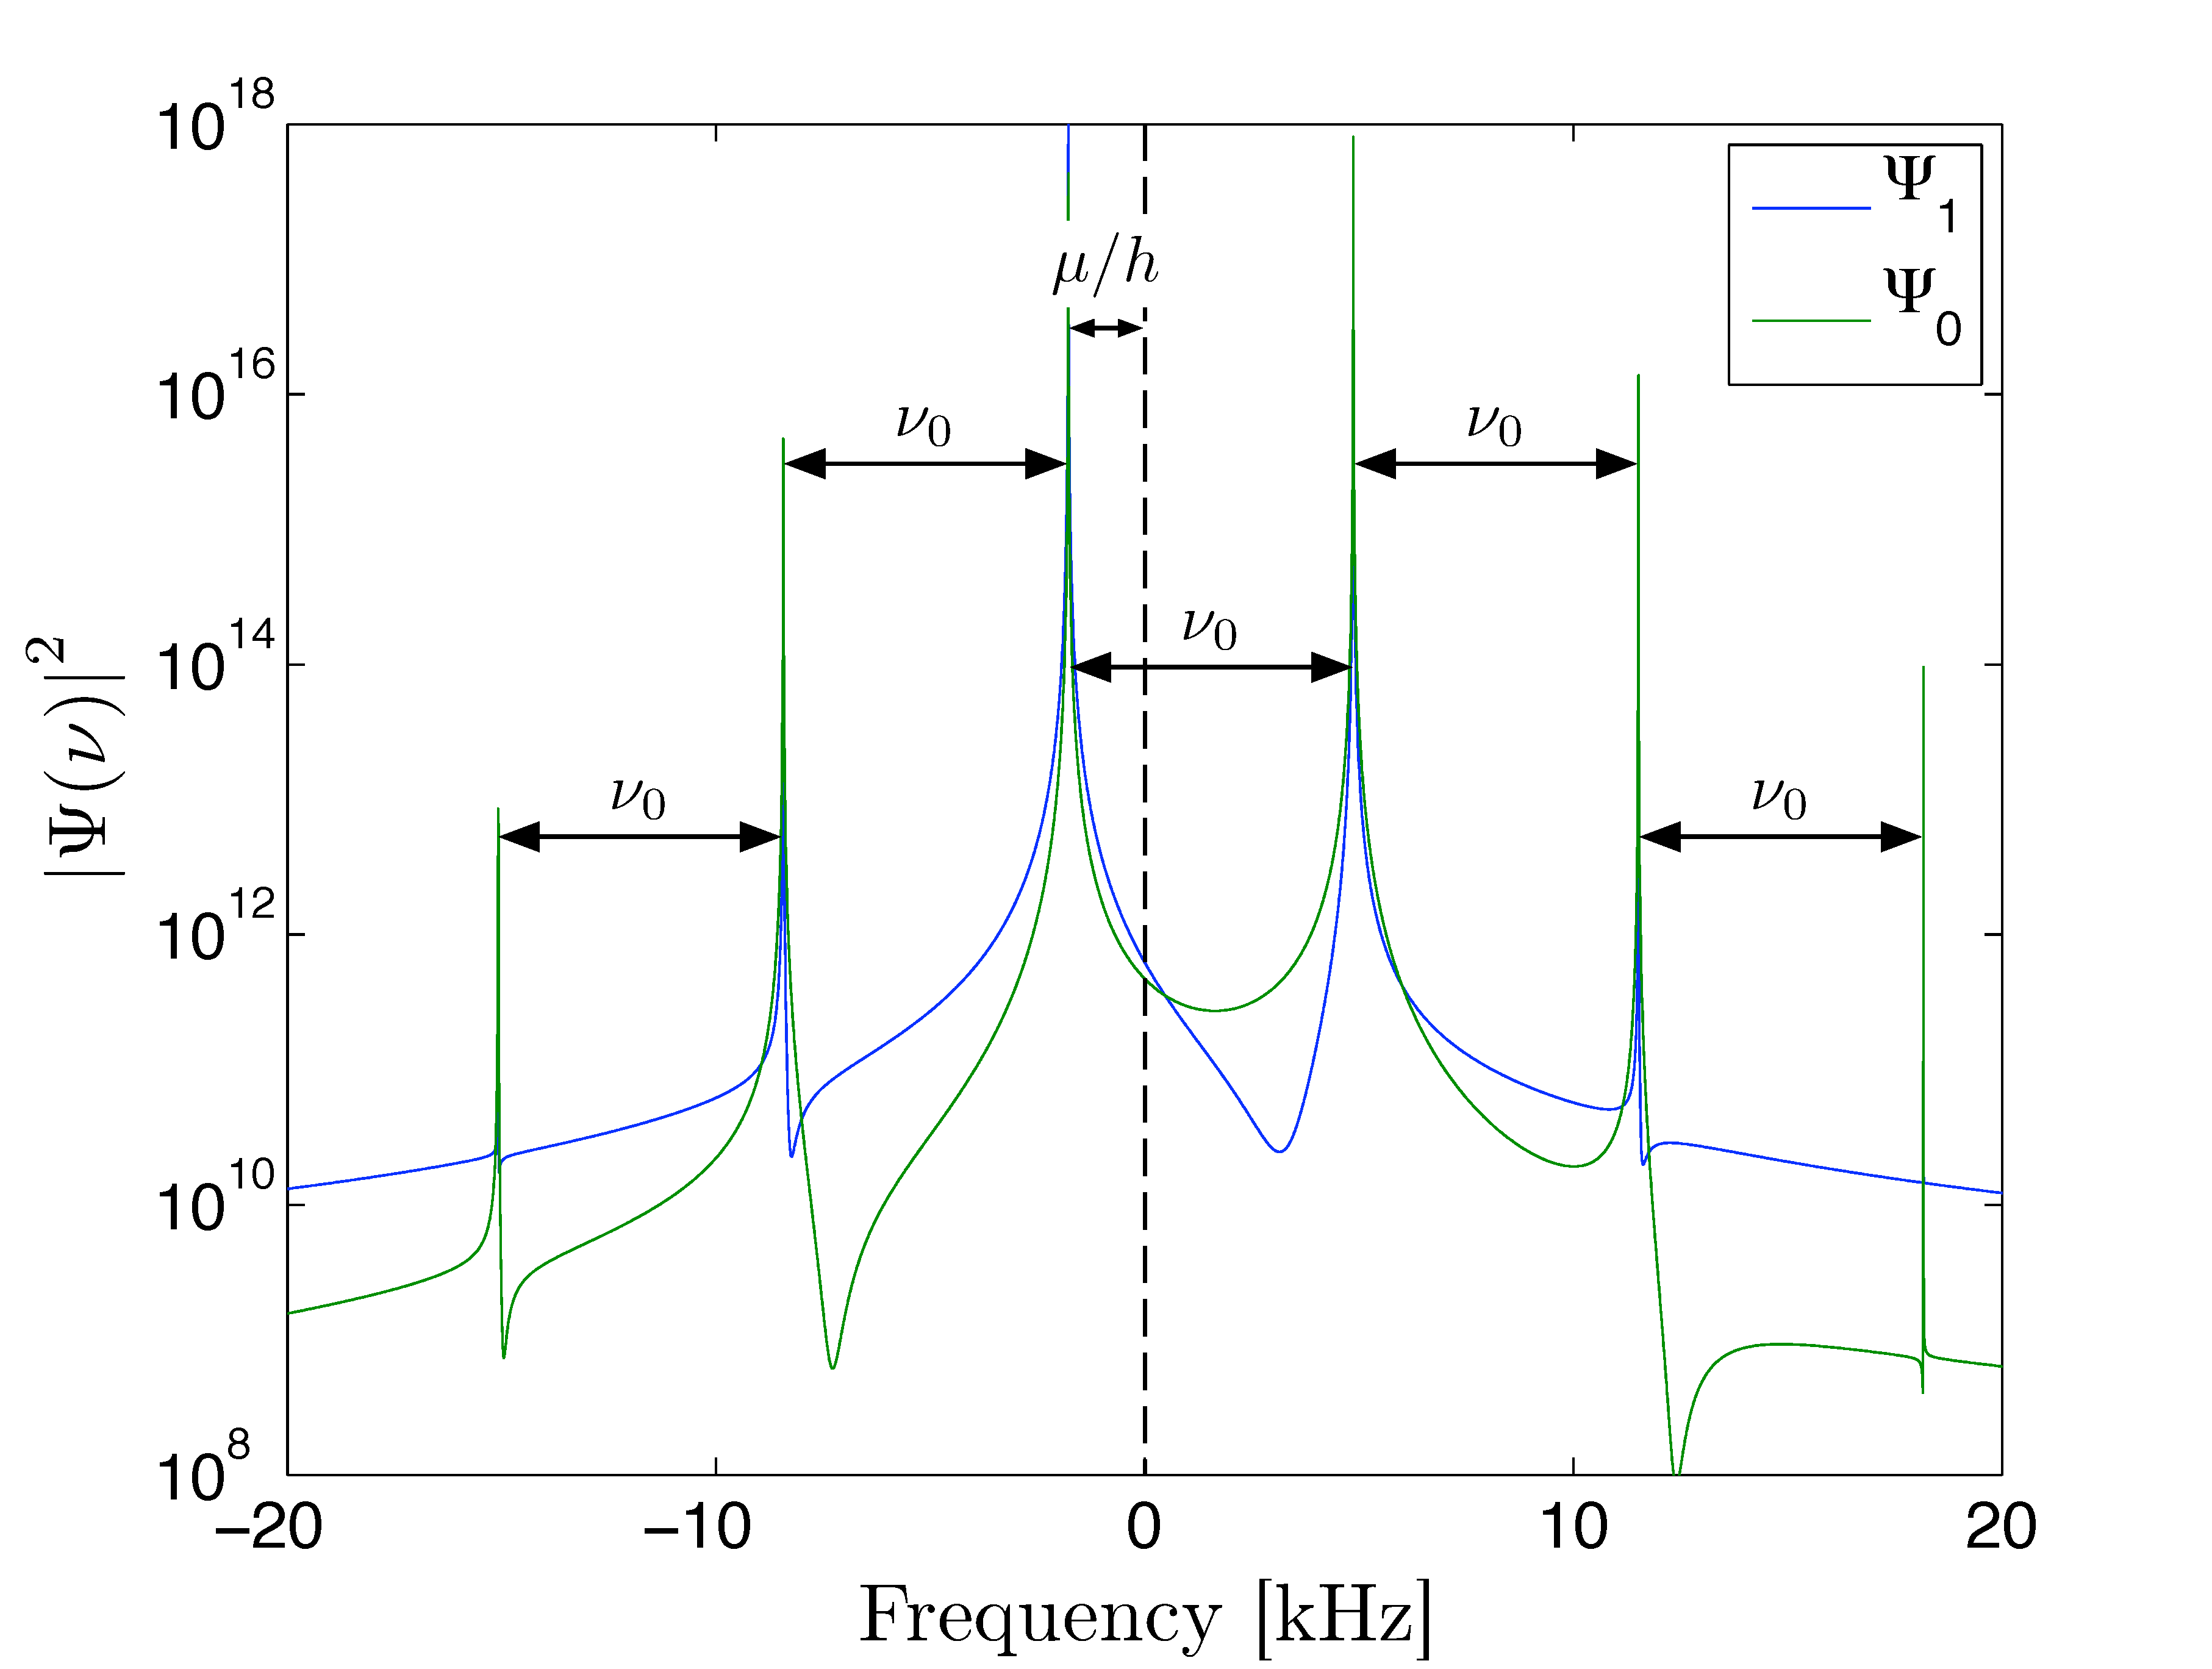
\includegraphics[width=14cm]{MeanFieldFourierTransform}
    \caption{\label{Peaks:MeanFieldFourierTransform} Temporal Fourier transform of the calculated mean field evolution defined by \eqref{Peaks:MeanFieldEquationsOfMotion} for the centre of the condensate defined by the experimental parameters given in \tableref{Peaks:ExperimentalParameters}. The frequency $\nu_0$ is the inverse period of the system, and $\Delta\nu$ represents the global phase rotation. From the data in this figure the values $\nu_0 = \unit[6.65]{kHz}$ and $\Delta\nu = \unit[-1.78]{kHz}$ can be determined, giving the period as $T=\unit[150]{\micro{}s}$.}
\end{figure}

The period and energy offset determined, it remains to calculate the mono\-dromy matrix $\mathcal{M}(\bm{k})$ from which the Floquet exponents may be derived. This is achieved by numerically solving the related matrix problem to \eqref{Peaks:DeviationOperatorsMatrixEvolution} from $t=0$ to $t=T$ [refer to \eqref{Peaks:MonodromyMatrix}]. Noting that the matrix $\mathcal{H}(\bm{k})$ only depends on $k = \abs{\bm{k}}$, the solutions for the Floquet exponents $\xi_i(\bm{k}) = \gamma_i(\bm{k}) + i\omega(\bm{k})$ are illustrated in \figureref{Peaks:CondensateEigenvalues}. 

\begin{figure}
    \centering
    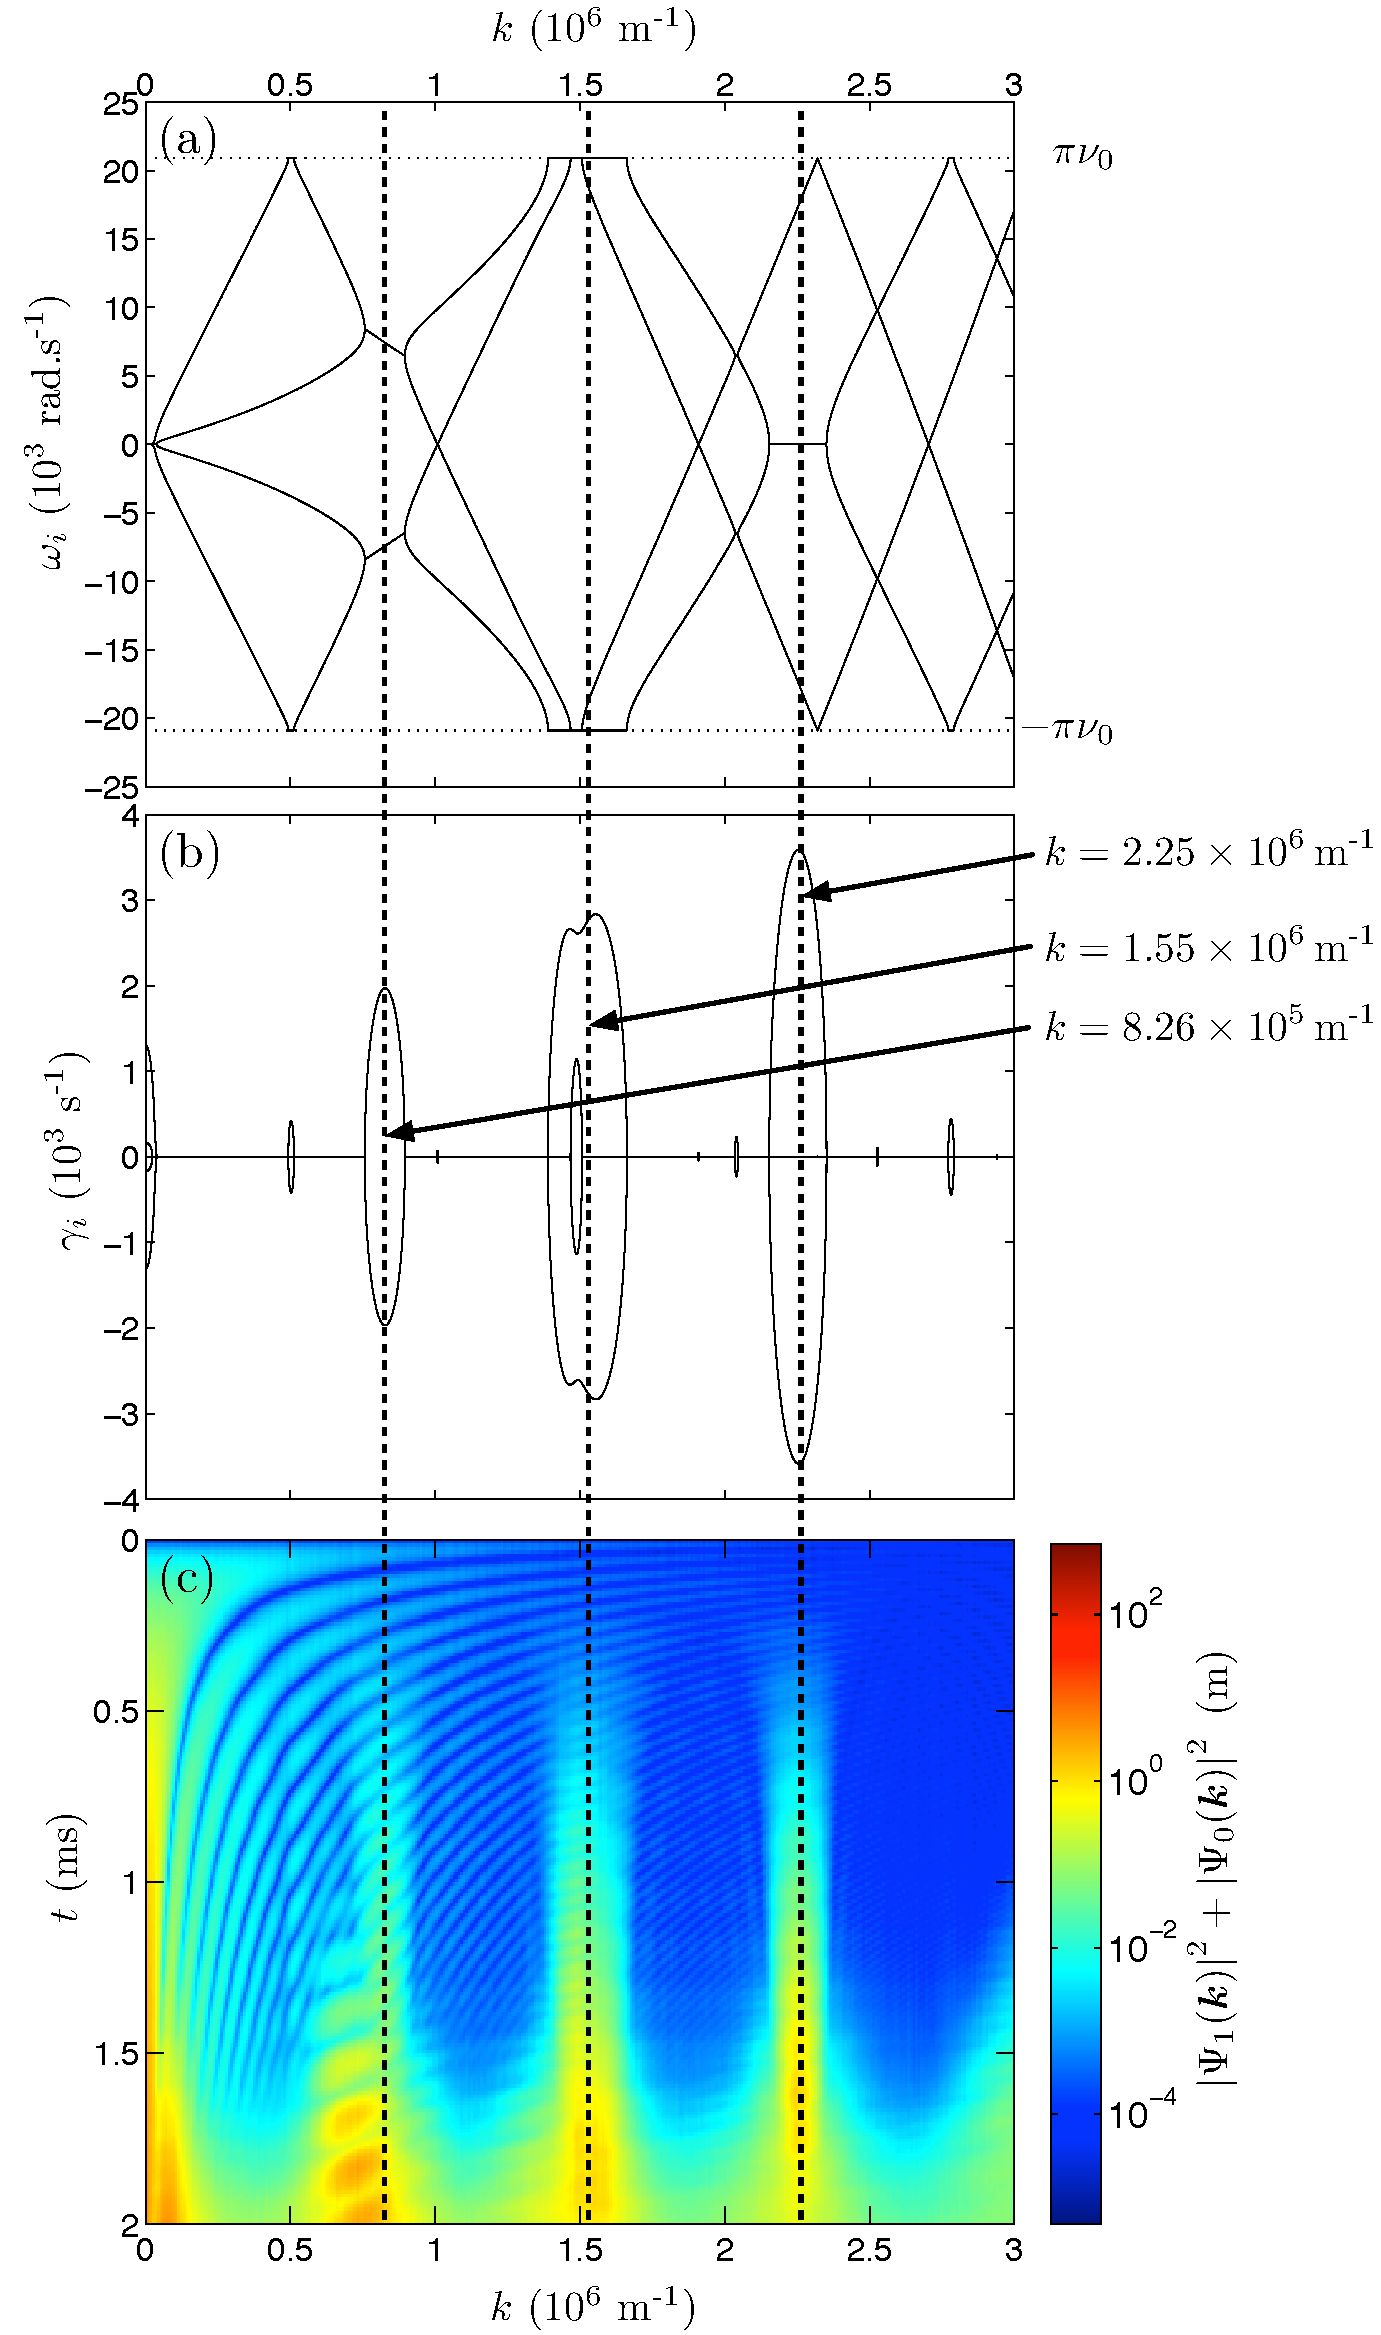
\includegraphics[height=19cm]{CondensateEigenvalues}
    \caption{\label{Peaks:CondensateEigenvalues}
        Illustration of the Floquet exponents for $\mathcal{H}(\bm{k})$ and comparison to a corresponding truncated Wigner simulation.
        Upper figure (a) displays the imaginary part $\omega_i$ of the Floquet exponents. As the $\omega_i$ can only be determined up to a multiple of $2\pi\nu_0$ [see \eqref{Peaks:AmbiguityFloquetExponent}], they have been reduced modulo $2\pi\nu_0$ into the range $\left[-\pi\nu_0,\, \pi\nu_0\right]$.
        The middle figure (b) shows the real part $\gamma_i$ of the Floquet exponents, which indicate an instability for the corresponding wavenumber when they are nonzero.
        Lower figure (c) shows the results of a 1D truncated Wigner simulation corresponding to the system under consideration in (a) and (b). The truncated Wigner simulation exhibits growth in the same modes predicted from the results of the perturbative analysis shown in (b). The truncated Wigner results shown are the average of 500 paths.}
\end{figure}

The temporal periodicity of the system implies that the imaginary components $\omega_i(\bm{k})$ of the Floquet exponents are only uniquely defined modulo $2\pi \nu_0$ (see \figureref{Peaks:CondensateEigenvalues}(a)). This is because any eigenvalue $\lambda$ of the monodromy matrix $\mathcal{M}(\bm{k})$ corresponds to infinitely many Floquet exponents,
\begin{align}
    \label{Peaks:AmbiguityFloquetExponent}
    \lambda = \exp\left[\left(\gamma + i\omega + i 2 \pi n \nu_0\right)T\right] = \exp\left[\left(\gamma + i \omega\right)T\right].
\end{align}
This does not hinder our understanding of the system as our primary interest is in the stability of the condensate to excitations, which is determined by the $\gamma_i(\bm{k})$.

The normalised eigenvectors of the system are not always annihilation or creation operators; as is discussed in \appendixref{PeaksAppendix}, this is only true when the Floquet exponents are pure imaginary. When the Floquet exponents have a nonzero real component, annihilation and creation operators can be constructed from linear combinations of the eigenvectors. Not being eigenvectors, these operators will therefore have nontrivial evolution. As is shown in \appendixref{PeaksAppendix}, Floquet exponents with nonzero real parts come in pairs of the form $\pm \gamma(\bm{k}) + i \omega(\bm{k})$. From the corresponding eigenvectors to these Floquet exponents the bosonic annihilation operator $\hat{\Lambda}(\bm{k}, t)$ can be formed, which evolves as
\begin{subequations}
    \label{Peaks:DynamicalInstability}
    \begin{align}
        \hat{\Lambda}(\bm{k}, nT) &= e^{i n\omega(\bm{k}) T} \left( \sinh(n\gamma(\bm{k}) T) \hat{\Lambda}'^\dagger(-\bm{k}, 0) + \cosh(n\gamma(\bm{k}) T) \hat{\Lambda}(\bm{k}, 0)\right),\\
        \hat{\Lambda}'(\bm{k}, nT) &= e^{-i n \omega(\bm{k}) T} \left( \sinh(n\gamma(\bm{k}) T) \hat{\Lambda}^\dagger(-\bm{k}, 0) + \cosh(n\gamma(\bm{k}) T) \hat{\Lambda}'(\bm{k}, 0)\right),
    \end{align}
\end{subequations}
where $n$ is a positive integer, and where $\hat{\Lambda}'(\bm{k}, t)$ will be equal to $\hat{\Lambda}(\bm{k}, t)$ in some circumstances discussed in \appendixref{PeaksAppendix}. Due to the exponential growth in \eqref{Peaks:DynamicalInstability}, the mode corresponding to $\hat{\Lambda}(\bm{k})$ represents a dynamical instability of the condensate.

The behaviour of the dynamical instabilities will be governed by \eqref{Peaks:DynamicalInstability} only while the unstable modes have a small occupation compared to the condensate, and scattering between the unstable modes can be neglected. \figureref{Peaks:CondensateEigenvalues}(c) shows the results of a truncated Wigner simulation of the Hamiltonian \eqref{Peaks:InitialHamiltonian}, which is in excellent agreement with the location of the dynamical instabilities as determined by the Floquet exponents [see \figureref{Peaks:CondensateEigenvalues}(b)]. For later times, there is an additional mode undergoing growth, $k \approx \unit[7.5\times 10^5]{m}^{-1}$. This mode is the result of scattering between the dynamical instabilities, a process neglected the perturbative approach taken in this section. 

\parasep

In summary, the procedure used to find the Floquet exponents of $\mathcal{H}(\bm{k})$, and hence the stability of the condensate to excitations is:
\begin{enumerate}
    \item Numerically solve \eqref{Peaks:MeanFieldEquationsOfMotion} with $\mu=0$ for a long period of time $t \gg T$ where $T$ is the periodicity of the solution.
    \item Perform the temporal Fourier transform of the solutions obtained for $\Psi_i(t)$ to accurately determine the period $T$ and the value of the energy offset $\mu$ required to cancel any global phase evolution to make the wavefunctions themselves periodic (see \figureref{Peaks:MeanFieldFourierTransform}).
    \item Using the calculated period and energy offset, numerically solve the related matrix problem to \eqref{Peaks:DeviationOperatorsMatrixEvolution} for a range of values of $\bm{k}$ to obtain the monodromy matrix $\mathcal{M}(\bm{k})$.
    \item Calculate the eigenvalues $\lambda_i$ of $\mathcal{M}(\bm{k})$ and determine the Floquet exponents $\xi_i$ using $\protect{\lambda_i = \exp(\xi_i T)}$ (see \figureref{Peaks:CondensateEigenvalues}).
\end{enumerate}

\subsection{Discussion of the dynamical instabilities}

The evolution of the dynamical instability $\hat{\Lambda}(\bm{k})$ given by \eqref{Peaks:DynamicalInstability} is equivalent to that of the non-degenerate parametric amplifier \citep{WallsMilburn}, which is a model for the parametric down-conversion of light by a non-linear crystal. In parametric down-conversion, two EPR\footnote{FIXME: EPR entanglement will need to be defined somewhere} entangled photons are produced at frequencies $\omega_1$ and $\omega_2$ with growth rate $\gamma$ from a classical seed beam at frequency $\omega = \omega_1 + \omega_2$. Analogously, in the case of the He* BEC discussed at the start of this chapter the evolution represented by \eqref{Peaks:DynamicalInstability} will result in the spontaneous formation of EPR entangled pairs of excitations, one in each of the $\hat{\Lambda}(\pm \bm{k})$ modes. Although these modes will be entangled upon production, it does not necessarily follow that parts of the outcoupled atom laser will be entangled; the entangled $\hat{\Lambda}(\bm{k})$ modes are each superpositions of $m_F=1$ and $m_F=0$ states, but only the $m_F=0$ atoms can leave the condensate. However, if the $m_F=1$ components of the entangled modes are assumed to be outcoupled faster than the time to reverse their momenta ($\unit[9]{ms}$), then number difference squeezing between the atom laser components with opposite axial momenta may be observed.

These excitations would not necessarily be expected to form along the tight trapping directions. Of the three most unstable modes in \figureref{Peaks:CondensateEigenvalues}, the shortest wavelength for these excitations is $\lambda \approx \unit[3]{\micro m}$ which is not significantly smaller than the Thomas-Fermi radius in this dimension of $\rho_\text{TF} = \unit[9.4]{\micro m}$. Hence the local density approximation will not be satisfied in this dimension as the condensate density decays to zero over this distance. However, as the Thomas-Fermi radius in the axial dimension is $z_\text{TF} = \unit[175]{\micro m}$, the local density approximation will be a good approximation for describing the excitations along that dimension.

This effect also depends on the scattering length for collisions between $m_F=0$ atoms being significantly smaller than both the 1--1 and 1--0 scattering lengths as no instabilities were found in the $\kappa = 1$ limit (see \sectionref{Peaks:Kappa1Limit}). 
Consequently, this effect would not be expected to be observed in atoms like $\nucl{87}{}{Rb}$.

Verification that the $\hat{\Lambda}(\bm{k})$ quasiparticles are the origin of the peak-like structure observed in the experiment required a full 3D field calculation to be discussed in \sectionref{Peaks:3DCalculation}.  The argument made in this section that the observed structure is due to the formation of pairs of quasiparticles formed via a spontaneous four-wave mixing process indicate that a Gross-Pitaevskii model will be unable to reproduce the observations. Such a mean-field model will be insufficient due to the absence of the vacuum fluctuations which are critical to all spontaneous processes.

\section{Full 3D calculation}
\label{Peaks:3DCalculation}

\subsection{Calculating Momentum Flux Density at the Edge of a Simulation Region}
When simulating a process the calculation region must include all of the interesting dynamics, however, unless a technique is used for removing 

without infinite calculational resources, a technique is required for 


When performing simulations the simulation region must contain the 


When performing simulations to model dynamics that occur over any significant timescale, 
